\section{Análisis formal de conceptos}
\subsection{Introducción}

El análisis formal de conceptos, FCA por sus siglas en inglés, es una teoría matemática basada en conceptos y jerarquías de conceptos que tiene como objetivo el descubrir estructuras conceptuales dentro de un conjunto de datos. Esta teoría queda definida por Rudolf Willie en 1982 y actualmente su eso está bastante extendido especialmente en problemas lingüísticos, como el procesamiento del lenguaje natural y la creación de bases de datos lingüísticas.

\subsection{Conceptos y contextos formales}

Como se ha dicho anteriormente, el FCA se basa en conceptos y jerarquías, desde un punto de vista lingüístico, un concepto se compone de dos partes, una de ellas es conjunto de objetos que pertenecen al concepto (Extensión) y la otra es una serie de atributos o propiedades que tienen todos los objetos anteriores (Intensión). En FCA se crea un modelo matemático del concepto que permite hablar de objetos, atributos y las relaciones entre ellos que nos permiten expresar que un objeto tiene un atributo. Este modelo es el contexto formal. \cite{A3}

El contexto formal es la forma utilizada en FCA para la representación de los datos y se define como un conjunto de la forma $K := (G,M,I)$ donde G, del alemán Gegenstande, es el conjunto de objetos. M, del alemán Merkmale, son los atributos e I son las relaciones binarias entre G y M (g tiene el atributo m). La representación más sencilla para un contexto formal es una matriz donde las filas se corresponden con el conjunto de objetos y las columnas se corresponden con el conjunto de atributos.


Un concepto formal del contexto formal $K := (G,M,I)$ queda definido como una tupla (A,B), donde A es un conjunto de objetos (Extensión) tal que $A \subseteq G$ y B es un conjunto de atributos (Intensión) tal que $B \subseteq M$, además se debe cumplir que $A = B'$ y $B = A'$ donde $A'$ y $B'$ son operadores de derivación tal que:
\begin{equation}
A' := \{m \in M \quad | \quad gIm \quad para \quad todo \quad g \in A\}
\end{equation}
\begin{equation}
B' := \{g \in M \quad | \quad gIm \quad para \quad todo \quad m \in B\}
\end{equation}
Como estos operadores forman una conexión de Galois, se cumplen las siguientes propiedades tanto para el conjunto A como para el conjunto B:

\begin{equation}
Z_{1} \subseteq Z_{2} \Longrightarrow Z_{1}' \supseteq Z_{2}'
\end{equation}
\begin{equation}
Z \subseteq Z''
\end{equation}
\begin{equation}
Z''' = Z'
\end{equation}

Además los conceptos se pueden ordenar, se considera que un objeto es mayor que otro cuando:
\begin{equation}
(A_{1},B_{1}) \leq (A_{2},B_{2}) : \Leftrightarrow A_{1} \subseteq A_{2}
\end{equation}
De esta forma decimos que $(A_{2},B_{2})$ es un superconcepto de $(A_{1},B_{1})$ y que $(A_{1},B_{1})$ es un subconcepto de $(A_{2},B_{2})$.


\subsection{Retícula}

La retícula es una forma de representar conocimiento en FCA de forma ordenada. Esta representación se realiza con un diagrama etiquetado, o diagrama de Hasse, un ejemplo de como es una retícula se puede ver en la figura \ref{fig:reticula}. Esta forma de representación no reduce los datos, por lo que tiene la ventaja de que mantiene todo el conocimiento descrito en el contexto formal y además permite visualizar la estructura conceptual que este conocimiento tiene
\cite{A5}.

En el diagrama, los nodos representan conceptos y las aristas representan relaciones entre conceptos, estas relaciones son del tipo A es subconcepto de B o A es superconcepto de B.

Si en un nodo aparece la etiqueta de un objeto \textit{g}, ese nodo representa el concepto más pequeño que contiene a \textit{g} en su extensión. Si aparece la etiqueta de un atributo \textit{m}, el nodo representa el concepto más grande que tiene a \textit{m} en su intensión. De esta forma, observando la retícula, podemos leer para un concepto (A,B) su extensión A y su intensión B.


%Al conjunto ordenado de todos los objetos de un contexto ($\mathfrak{B}(G,M,I)$) se lo conoce como retícula del contexto. La retícula se define con el siguiente teorema:
%
%Para un conjunto $\{(A_{i},B_{i}) | i \in I\} \subseteq \mathfrak{B}(G,M,I)$ de conceptos formales, el supremo ($\top$) viene dado por:
%\begin{equation}
%\bigvee (A_{i},B_{i}) = ((\bigcup A_{i})^{n}, \bigcap B_{i})
%\end{equation}
%y el ínfimo ($\bot$) por:
%\begin{equation}
%\bigwedge (A_{i},B_{i}) = (\bigcap A_{i}, (\bigcup B_{i})^{n})
%\end{equation}
\subsection{Reglas de asociación}

Las reglas de asociación son una proposición probabilística que se utilizan para describir hechos que se dan dentro de un conjunto de datos, en este caso dentro del contexto formal. Este tipo de reglas puede verse de la forma SI \textit{X} ENTONCES \textit{Y}, donde \textit{X} es el antecedente o parte izquierda de la regla e \textit{Y} es el consecuente o parte derecha de la regla\cite{B2}. Una regla puede tener uno o varios antecedentes o consecuentes, para unir estos elementos se hace uso de los operadores de conjunción (AND) y disyunción (OR). Los parámetros que definen una regla son los siguientes:

Soporte, esta medida refleja cuanto objetos apoyan el antecedente o el consecuente de la regla.
Confianza, la confianza refleja en tanto por ciento cuantos objetos que apoyan en antecedente cumplen el consecuente.

\subsection{Concept Explorer}
Concept Explorer es la herramienta que hemos utilizado cargar el contexto que vamos a generar y  obtener las reglas de asociación que posteriormente utilizaremos en la fase de clasificación. Además podremos visualizar la jerarquía de nuestro contexto. 
\subsubsection{Creación del contexto formal}
Para la creación de un contexto $K := (G,M,I)$ necesitamos definir un conjunto de atributos (M) y un conjunto de objetos (G). Como atributos hemos tomado un conjunto de palabras extraídas de las noticias formado por las palabras más comunes de cada categoría de noticias. Como conjunto de objetos tenemos el texto de un número determinado de noticias de cada categoría. 

El proceso que hemos seguido para especificar las relaciones entre objetos y atributos (I) es el siguiente, lo primero es generar el conjunto de atributos como está descrito en la sección \nameref{sec:atributos}. Para obtener el conjunto de objetos hacemos consultas a la base de datos para obtener, de cada categoría, un subconjunto de noticias seleccionadas de manera aleatoria. Una vez hemos determinado ambos conjuntos, tomamos el texto y la lista de atributos y recorremos la lista comprobando si el elemento está en el texto si está lo señalamos en el fichero con una X y sino con un punto.

El contexto creado se guarda con un fichero de extensión ''.cxt'' generado de manera automática. La estructura de un fichero de contexto es la siguiente:
\begin{lstlisting}
B

46
90

64110
112609
68691
  .
  .
  .
  .
68693
sector
cobre
cultura
sociales
agricultura
empleo
  .
  .
  .
  .
seguridad
actividades
ETIQUETA_turismo1
ETIQUETA_ssociales
ETIQUETA_recursosHumanos
ETIQUETA_obras
ETIQUETA_igualdad
ETIQUETA_Mujer
  .
  .
  .
  
ETIQUETA_mayores
ETIQUETA_rtv
ETIQUETA_cont
..X...........X...X......X..XX..X....XX..........X..X.............X...X..........X........
...X......XX...X.....................X.X..................................................
.....XX............................X...XXX.X..XX.XX.X......XX.....X...X..X.......X........
......X...................X..............X................................................
...X.......................................X..............................................
.......X..X......X..............X....X......X.............................................

\end{lstlisting}

El contexto queda representado en Concept Explorer de la siguiente manera:

\begin{center}
\begin{figure}[h]

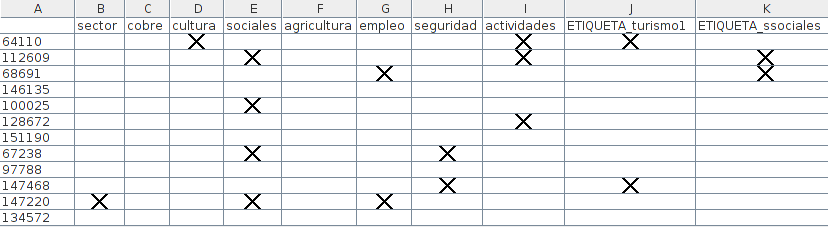
\includegraphics[scale=0.5]{fca/contexto.png}
\caption{Representación del contexto obtenido}
\label{fig:reticula}
\end{figure}
\end{center}
\subsubsection{Creación del retículo}
Otra de las posibilidades que ofrece FCA es la representación del contexto y de las relaciones entre objetos y atributos, estas relaciones son conocidas como relaciones de Galois. Como durante la realización del proyecto hemos generado contexto con un número alto de atributos y objetos la representación del retículo no se puede visualizar de forma clara.
Aún así es posible obtener una representación simplificada reduciendo el número de objetos, el retículo obtenido se muestra en la figura \ref{fig:contexto}.
\begin{center}
\begin{figure}

\hspace*{-3cm}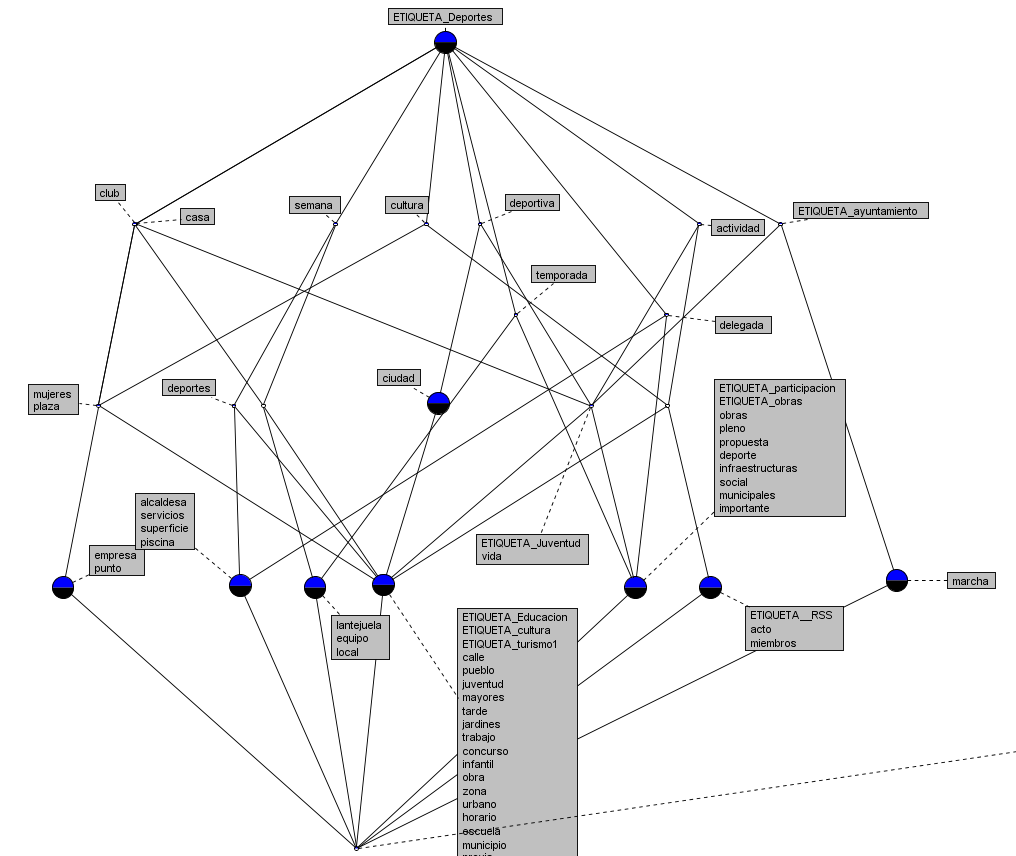
\includegraphics[scale=0.83]{fca/lattice_deportes.png}
\caption{Representación del contexto obtenido}
\label{fig:contexto}
\end{figure}
\end{center}
\subsection{Experimentación}

Para determinar como afecta el tamaño de los conjuntos de objetos y atributos a la precisión del clasificador hemos realizado pruebas con diferentes tamaños de conjuntos con los valores indicados en la siguiente tabla:
\vspace{1em}
\begin{center}

\begin{tabular}{|c|c|c|}
  \hline 
  Experimento & Número de objetos & Número de atributos \\ 
  \hline 
  Experimento 1 & 133 & 145 \\ 
  \hline 
  Experimento 2 & 258 & 208 \\ 
  \hline 
  Experimento 3 & 372 & 257 \\ 
  \hline 
  \end{tabular}   
  
\end{center}
\vspace{1em}

Con la herramienta Concept Explorer generamos reglas de asociación en base Stem. Para generar el fichero .clp que necesitamos para la fase de clasificación utilizamos un código Java escrito por Gonzalo Aranda para leer las reglas obtenidas en Concept Explorer y generar el fichero de salida. Este código ha sido modificado para tener en cuenta una serie de restricciones del problema. La primera es eliminar aquellas reglas con un soporte igual a cero, ya que no tienen ningún objeto que las cumpla. También eliminamos aquellas reglas que en su parte izquierda no tengan una etiqueta de alguna categoría ya que no nos aportan información útil en nuestro estudio.

Durante la experimentación se obtuvieron los siguientes números de reglas:

\vspace{1em}
\begin{tabular}{|c|c|c|}
\hline 
Experimentos & Número de reglas obtenidas & Número de reglas válidas \\ 
\hline 
Experimento 1 & 7412 & 2650 \\ 
\hline 
Experimento 2 & 26344 & 9813 \\ 
\hline 
Experimento 3 & 66910 & 53898 \\ 
\hline 
\end{tabular} 
\vspace{1em} 

La regla \textless 3 \textgreater talleres desarrollo proyecto =[100\%]=\textgreater \textless 3 \textgreater actividades; no es una regla válida por no tener una etiqueta en el consecuente y la regla \textless 2 \textgreater delegado sanidad =[100\%]=\textgreater \textless 2 \textgreater salud objetivo ETIQUETA\_consumo ETIQUETA\_salud se considera correcta.

